\chapter{Épidémiologie de la Chikungunya}


\section*{Introduction}

 
\section{Origine de la Chikungunya}
\textbf{Chikungunya fever} (CHIKF) is a viral disease that was first described in \textbf{1952} during an outbreak in southern Tanzania. The name comes from a word in the \textit{Makonde} language, spoken in southeast Tanzania and northern Mozambique, that means "\textit{to become contorted}" or "\textit{that which bends up}". The virus was first isolated in Thailand in 1958.\cite{origin}

\section{Agent Pathogène}

Blajxckc

\subsection{Le virus Chikungunya}

\begin{figure}[!h]
	\begin{center}
		%taille de l'image en largeur
		%remplacer "width" par "height" pour régler la hauteur
		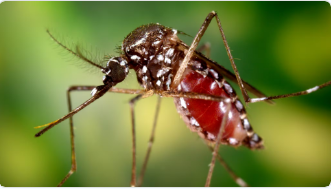
\includegraphics[width=10cm]{images/moustique}
	\end{center}
	%légende de l'image
	\caption{Aedes aegypti mosquito full of blood}
	\label{fig:aedes}
\end{figure}

\begin{figure}[!h]
	\begin{center}
		%taille de l'image en largeur
		%remplacer "width" par "height" pour régler la hauteur
		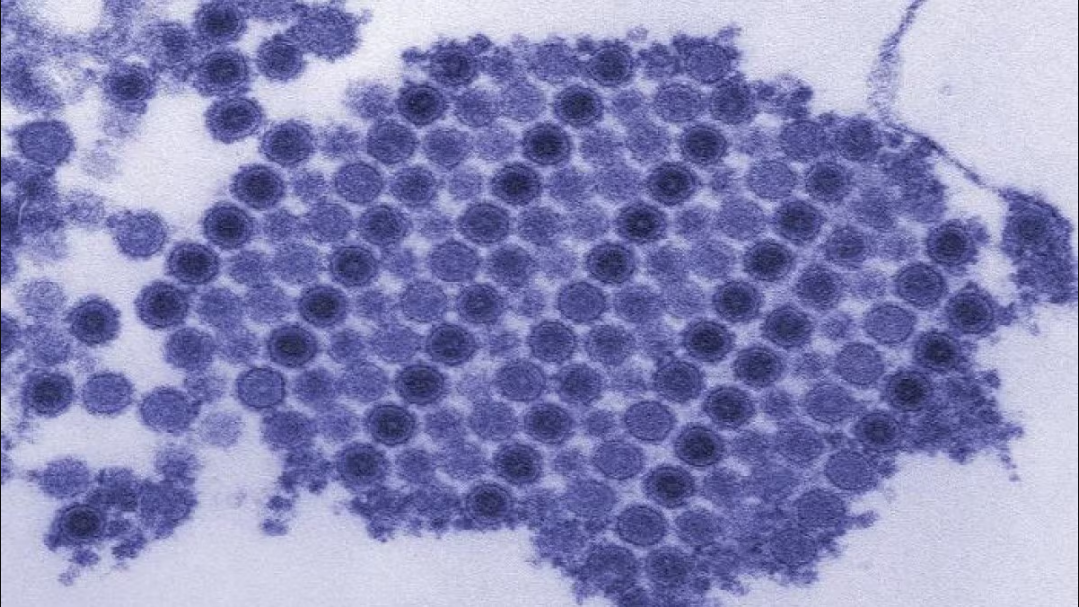
\includegraphics[width=10cm]{images/CHIK_17550_TEM}
	\end{center}
	%légende de l'image
	\caption{Electron microscopic image of chikungunya virus}
	\label{fig:chikv}
\end{figure}

\begin{figure}[!h]
	\begin{center}
		%taille de l'image en largeur
		%remplacer "width" par "height" pour régler la hauteur
		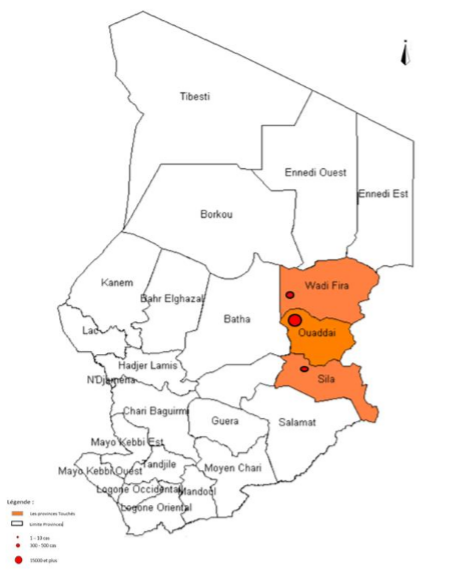
\includegraphics[width=10cm]{images/chadmap}
	\end{center}
	%légende de l'image
	\caption{Tools to Develop our Model}
	\label{Tools to Develop our Model}
\end{figure}

\begin{figure}[!h]
	\begin{center}
		%taille de l'image en largeur
		%remplacer "width" par "height" pour régler la hauteur
		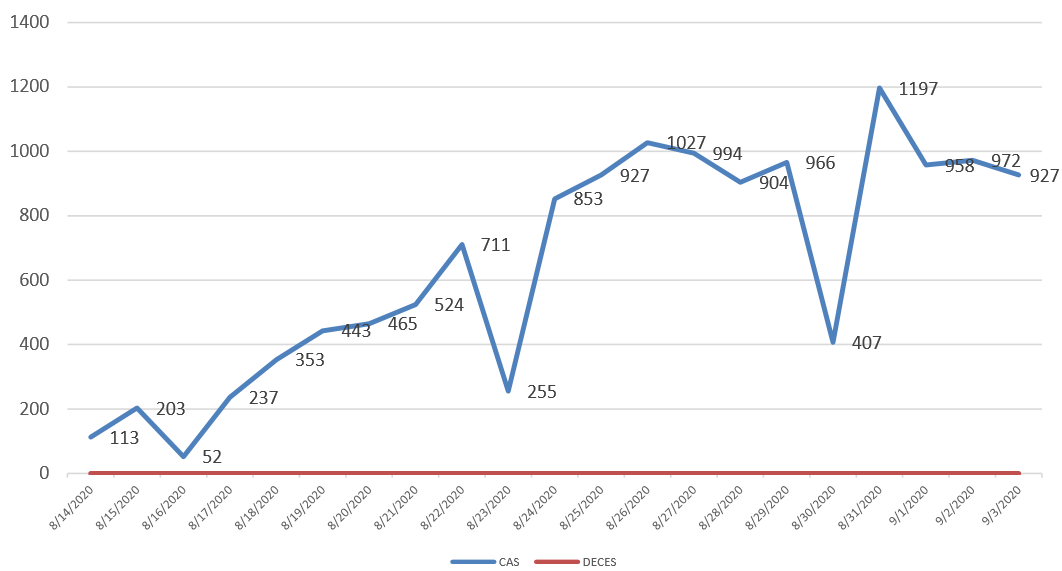
\includegraphics[width=10cm]{images/statsCaseChad}
	\end{center}
	%légende de l'image
	\caption{Tools to Develop our Model}
	\label{Tools to Develop our Model}
\end{figure}

\begin{figure}[!h]
	\begin{center}
		%taille de l'image en largeur
		%remplacer "width" par "height" pour régler la hauteur
		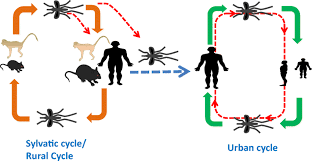
\includegraphics[width=10cm]{images/trans}
	\end{center}
	%légende de l'image
	\caption{Tools to Develop Model}
	\label{Tools to Develop our Model}
\end{figure}

\begin{figure}[!h]
	\begin{center}
		%taille de l'image en largeur
		%remplacer "width" par "height" pour régler la hauteur
		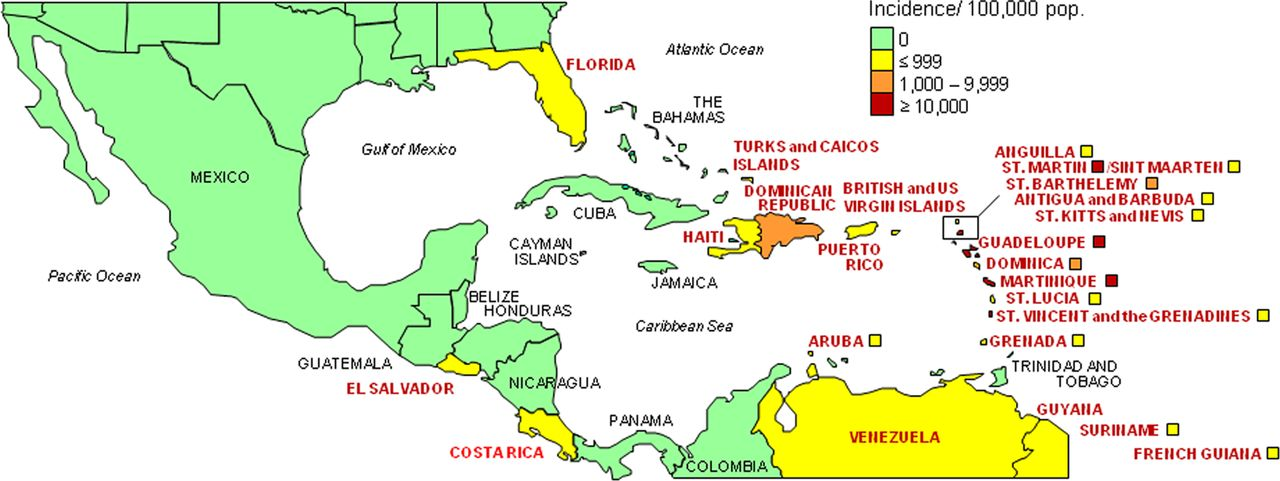
\includegraphics[width=10cm]{images/zjv9990995820001}
	\end{center}
	%légende de l'image
	\caption{Tools to Develop our Model}
	\label{Tools to Develop our Model}
\end{figure}
\section{Mode de Transmission}

Bla

\subsection{Vecteurs : Les moustiques Aedes}

Bla

\subsection{La transmission}
Le \textbf{CHIKV} se transmet selon deux cycles différents :
\begin{itemize}
	\item \textbf{Cycle urbain} : transmission de l'homme au moustique.
	\item \textbf{Cycle sylvatique} : transmission de l'animal au moustique, puis à l'homme \cite{ganesan2017chikungunya}.
\end{itemize}
Le cycle sylvatique est la principale forme de transmission en Afrique \cite{ganesan2017chikungunya}. Ailleurs, dans les zones plus densément peuplées, le CHIKV se maintient principalement dans un cycle urbain, dans lequel les humains sont les principaux hôtes et les moustiques du genre \textit{Aedes} les vecteurs \cite{ganesan2017chikungunya} (voir figure\ref).
bien que \textit{Ae. aegypti} continue d'être un vecteur viral important, comme on l'a vu lors de la flambée épidémique dans les Caraïbes en 2013 \cite{ganesan2017chikungunya}.

La transmission verticale de la mère à l'enfant a été postulée pour expliquer les incidences postérieures à 2005 \cite{ganesan2017chikungunya}, étant particulièrement délétère lorsque :
\begin{itemize}
	\item la mère est infectée jusqu'à quatre jours après l'accouchement \cite{ganesan2017chikungunya},
\end{itemize}
bien que cette hypothèse ait été contestée \cite{ganesan2017chikungunya}.

\section{Symptômes et Diagnostic}
La reconnaissance des symptômes et l'établissement d'un diagnostic précis sont essentiels pour la gestion efficace des cas de chikungunya. Cette section examine les manifestations cliniques typiques de l'infection par le virus chikungunya ainsi que les méthodes diagnostiques utilisées pour identifier la maladie.
\subsection{Symptômes}
Chez les patients symptomatiques, la maladie à \textbf{CHIKV} se déclare généralement 4 à 8 jours (entre 2 et 12 jours) après la piqûre d'un moustique infecté. Elle se caractérise par une brusque poussée de fièvre, souvent accompagnée de fortes douleurs articulaires. Les douleurs articulaires sont souvent invalidantes et durent généralement quelques jours, mais peuvent être prolongées et durer des semaines, des mois, voire des années. D'autres signes et symptômes courants sont le gonflement des articulations, les douleurs musculaires, les maux de tête, les nausées, la fatigue et les éruptions cutanées. Comme ces symptômes se confondent avec ceux d'autres infections, notamment celles dues aux virus de la dengue et du Zika, les cas peuvent être mal diagnostiqués. En l'absence de douleurs articulaires importantes, les symptômes des personnes infectées sont généralement légers et l'infection peut passer inaperçue.

La plupart des patients se rétablissent complètement de l'infection ; toutefois, des cas occasionnels de complications oculaires, cardiaques et neurologiques ont été signalés dans le cadre d'infections par le \textbf{CHIKV}. Les patients situés aux extrémités du spectre d'âge sont plus exposés à une maladie grave. Les nouveau-nés infectés pendant l'accouchement et les personnes âgées souffrant de pathologies sous-jacentes peuvent devenir gravement malades et l'infection par le \textbf{CHIKV} peut augmenter le risque de décès~\cite{who2}.

Une fois qu'une personne est guérie, les données disponibles suggèrent qu'elle est probablement immunisée contre les infections futures~\cite{auerswald2018broad}.

\subsection{Méthodes de diagnostic}
ccxc
Bla

\section{Méthodes de Contrôle et Traitement}

La gestion efficace de l'épidémie de chikungunya repose sur une combinaison de stratégies de contrôle des vecteurs et d'interventions médicales. Cette section explore les diverses approches utilisées pour prévenir la transmission du virus et traiter les symptômes chez les patients infectés.

\subsection{Méthodes de contrôle}

Bla

\subsection{Options de traitement}

Bla

\section{Cas du Tchad}

L'analyse spécifique des cas de chikungunya au Tchad permet de comprendre l'impact de cette maladie dans un contexte régional spécifique. Cette section examine les caractéristiques épidémiologiques, les stratégies de contrôle et les défis rencontrés dans la gestion de l'infection par le virus chikungunya dans ce pays d'Afrique centrale.
\subsection{Facteurs climatiques influençant la propagation}

Bla

\subsection{Études de cas et données climatiques}
